\documentclass[lualatex,handout]{beamer}
\setbeamertemplate{footline}[frame number]
\usepackage{luatexja}
\usepackage{amsmath,amssymb}

\usepackage{tikz}
\usepackage{pgfplots}
\pgfplotsset{compat=1.18}

%\usepackage[haranoaji]{luatexja-preset}
\usepackage[deluxe,ipaex]{luatexja-preset}
\renewcommand{\kanjifamilydefault}{\gtdefault}
%\setmainjfont{HaranoAjiGothic-Regular}

\usepackage{unicode-math}
%\setmathfont{Fira Math}
\setmathfont{STIX Two Math}
\setmathrm{STIX Two Math}[StylisticSet=8]

%\usefonttheme{professionalfonts}

\usepackage{luacolor}

\newcommand{\emm}[1]{\textcolor{red}{#1}}
\newcommand{\expt}[1]{\mathbb{E}\left[#1\right]}
\newcommand{\var}[1]{\mathbb{V}\left[#1\right]}
\newcommand{\cov}[1]{\mathrm{Cov}\left[#1\right]}


\usepackage{xspace}
\newcommand\bm[1]{{\mathbf{#1}}}
\newcommand\dx{{\,\mathrm{d}x}}

\theoremstyle{definition}

\title{確率・統計基礎: 集中不等式}
\author{森 立平}
\date{}



\begin{document}
\begin{frame}[plain]
\maketitle
\end{frame}

\begin{frame}{集中不等式}
$N$個の独立な確率変数の和が期待値周辺に集中するという

独立同分布(independently and identically distributed (i.i.d.))
\end{frame}

\begin{frame}{二項分布}
\begin{align*}
\Pr(X = k) &= \binom{n}{k} p^k(1-p)^{n-k},\quad \emm{n=30},\, p=0.3.
\end{align*}
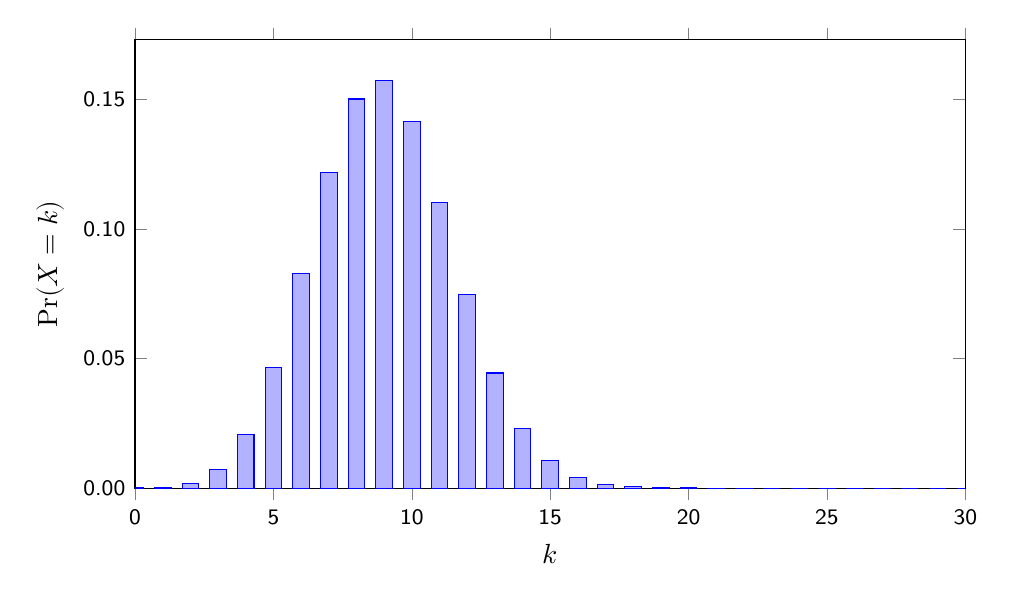
\begin{tikzpicture}[%
declare function={binom(\k,\n,\p)=\n!/(\k!*(\n-\k)!)*\p^\k*(1-\p)^(\n-\k);}]
\pgfmathsetmacro{\binomN}{30}
\begin{axis}[
    width=\textwidth, height=\axisdefaultheight,
    ylabel={$\Pr(X=k)$},
    xlabel={$k$},
    xmin=0, xmax=\binomN,
    ymin=0,
    scaled ticks = false,
    tick label style={/pgf/number format/assume math mode=true, font=\footnotesize\sffamily},
    yticklabel style={/pgf/number format/.cd, fixed, fixed zerofill, precision=2},
        domain=0:\binomN,samples at={0,1,...,\binomN},
    mark options={scale=0.75, blue},
    ybar, bar width = 6pt
        ]
%\addplot[ycomb] {binom(x,\binomN,0.3)};
\addplot {binom(x,\binomN,0.3)};
\end{axis}
\end{tikzpicture}
\end{frame}

\begin{frame}{二項分布}
\begin{align*}
\Pr(X = k) &= \binom{n}{k} p^k(1-p)^{n-k},\quad \emm{n=60},\, p=0.3.
\end{align*}
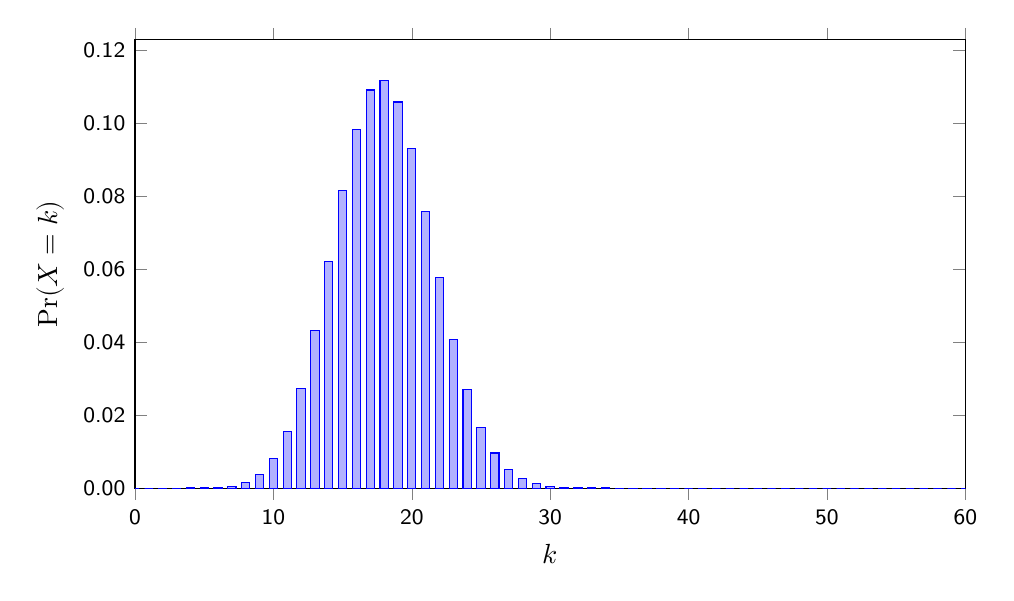
\begin{tikzpicture}[%
declare function={binom(\k,\n,\p)=\n!/(\k!*(\n-\k)!)*\p^\k*(1-\p)^(\n-\k);}]
\pgfmathsetmacro{\binomN}{60}
\begin{axis}[
    width=\textwidth, height=\axisdefaultheight,
    ylabel={$\Pr(X=k)$},
    xlabel={$k$},
    xmin=0, xmax=\binomN,
    ymin=0,
    scaled ticks = false,
    tick label style={/pgf/number format/assume math mode=true, font=\footnotesize\sffamily},
    yticklabel style={/pgf/number format/.cd, fixed, fixed zerofill, precision=2},
        domain=0:\binomN,samples at={0,1,...,\binomN},
    mark options={scale=0.75, blue},
    ybar, bar width = 3pt
        ]
%\addplot[ycomb] {binom(x,\binomN,0.3)};
\addplot {binom(x,\binomN,0.3)};
\end{axis}
\end{tikzpicture}
\end{frame}

\begin{frame}{二項分布}
\begin{align*}
\Pr(X = k) &= \binom{n}{k} p^k(1-p)^{n-k},\quad \emm{n=120},\, p=0.3.
\end{align*}
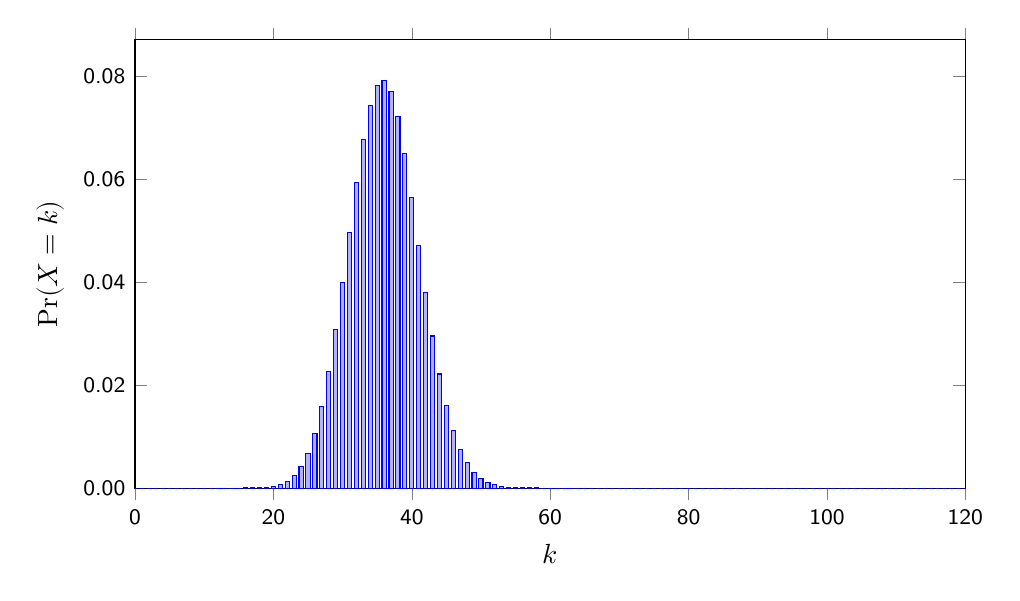
\begin{tikzpicture}[%
declare function={binom(\k,\n,\p)=\n!/(\k!*(\n-\k)!)*\p^\k*(1-\p)^(\n-\k);}]
\pgfmathsetmacro{\binomN}{120}
\begin{axis}[
    width=\textwidth, height=\axisdefaultheight,
    ylabel={$\Pr(X=k)$},
    xlabel={$k$},
    xmin=0, xmax=\binomN,
    ymin=0,
    scaled ticks = false,
    tick label style={/pgf/number format/assume math mode=true, font=\footnotesize\sffamily},
    yticklabel style={/pgf/number format/.cd, fixed, fixed zerofill, precision=2},
        domain=0:\binomN,samples at={0,1,...,\binomN},
    mark options={scale=0.75, blue},
    ybar, bar width = 1.5pt
        ]
%\addplot[ycomb] {binom(x,\binomN,0.3)};
\addplot {binom(x,\binomN,0.3)};
\end{axis}
\end{tikzpicture}
\end{frame}

\begin{frame}{二項分布}
\begin{align*}
\Pr(X = k) &= \binom{n}{k} p^k(1-p)^{n-k},\quad \emm{n=240},\, p=0.3.
\end{align*}
\begin{tikzpicture}[%
declare function={binom(\k,\n,\p)=\n!/(\k!*(\n-\k)!)*\p^\k*(1-\p)^(\n-\k);}]
\pgfmathsetmacro{\binomN}{240}
\pgfmathsetmacro{\p}{0.3}
\begin{axis}[
    width=\textwidth, height=\axisdefaultheight,
    ylabel={$\Pr(X=k)$},
    xlabel={$k$},
    xmin=0, xmax=\binomN,
    ymin=0,
    scaled ticks = false,
    tick label style={/pgf/number format/assume math mode=true, font=\footnotesize\sffamily},
    yticklabel style={/pgf/number format/.cd, fixed, fixed zerofill, precision=2},
        domain=0:\binomN,samples at={0,1,...,\binomN},
    mark options={scale=0.75, blue},
    ybar, bar width = .75pt
        ]
%\addplot[ycomb] {binom(x,\binomN,0.3)};
%\addplot {binom(x,\binomN,0.3)};
\addplot[domain=0:\binomN, color=blue, samples={\binomN+1}, thick] gnuplot { exp(lgamma(\binomN+1) - lgamma(x+1) - lgamma(\binomN-x+1) + x*log(\p) + (\binomN-x)*log(1-\p)) with impulses};
\end{axis}
\end{tikzpicture}
\end{frame}

\begin{frame}{二項分布}
\begin{align*}
\Pr(X = k) &= \binom{n}{k} p^k(1-p)^{n-k},\quad \emm{n=480},\, p=0.3.
\end{align*}
\begin{tikzpicture}[%
declare function={binom(\k,\n,\p)=\n!/(\k!*(\n-\k)!)*\p^\k*(1-\p)^(\n-\k);}]
\pgfmathsetmacro{\binomN}{480}
\pgfmathsetmacro{\p}{0.3}
\begin{axis}[
    width=\textwidth, height=\axisdefaultheight,
    ylabel={$\Pr(X=k)$},
    xlabel={$k$},
    xmin=0, xmax=\binomN,
    ymin=0,
    scaled ticks = false,
    tick label style={/pgf/number format/assume math mode=true, font=\footnotesize\sffamily},
    yticklabel style={/pgf/number format/.cd, fixed, fixed zerofill, precision=2},
        domain=0:\binomN,samples at={0,1,...,\binomN},
    mark options={scale=0.75, blue},
    ybar, bar width = .375pt
        ]
%\addplot[ycomb] {binom(x,\binomN,0.3)};
%\addplot {binom(x,\binomN,0.3)};
\addplot[domain=0:\binomN, color=blue, samples={\binomN+1}, thick] gnuplot { exp(lgamma(\binomN+1) - lgamma(x+1) - lgamma(\binomN-x+1) + x*log(\p) + (\binomN-x)*log(1-\p)) with impulses};
%\addplot[domain=0:\binomN, thick] gnuplot {x};
\end{axis}
\end{tikzpicture}
\end{frame}

\begin{frame}{二項分布}
\begin{align*}
\Pr(X = k) &= \binom{n}{k} p^k(1-p)^{n-k},\quad \emm{n=1000},\, p=0.3.
\end{align*}
\begin{tikzpicture}[%
declare function={binom(\k,\n,\p)=\n!/(\k!*(\n-\k)!)*\p^\k*(1-\p)^(\n-\k);}]
\pgfmathsetmacro{\binomN}{1000}
\pgfmathsetmacro{\p}{0.3}
\begin{axis}[
    width=\textwidth, height=\axisdefaultheight,
    ylabel={$\Pr(X=k)$},
    xlabel={$k$},
    xmin=0, xmax=\binomN,
    ymin=0,
    scaled ticks = false,
    tick label style={/pgf/number format/assume math mode=true, font=\footnotesize\sffamily},
    yticklabel style={/pgf/number format/.cd, fixed, fixed zerofill, precision=2},
        domain=0:\binomN,samples at={0,1,...,\binomN},
    mark options={scale=0.75, blue},
    ybar, bar width = .375pt
        ]
%\addplot[ycomb] {binom(x,\binomN,0.3)};
%\addplot {binom(x,\binomN,0.3)};
\addplot[domain=0:\binomN, color=blue, samples={\binomN+1}, thick] gnuplot { exp(lgamma(\binomN+1) - lgamma(x+1) - lgamma(\binomN-x+1) + x*log(\p) + (\binomN-x)*log(1-\p)) with impulses};
%\addplot[domain=0:\binomN, thick] gnuplot {x};
\end{axis}
\end{tikzpicture}
\end{frame}

\begin{frame}{二項分布}
\begin{align*}
\Pr(X = k) &= \binom{n}{k} p^k(1-p)^{n-k},\quad \emm{n=10000},\, p=0.3.
\end{align*}
\begin{tikzpicture}[%
declare function={binom(\k,\n,\p)=\n!/(\k!*(\n-\k)!)*\p^\k*(1-\p)^(\n-\k);}]
\pgfmathsetmacro{\binomN}{10000}
\pgfmathsetmacro{\p}{0.3}
\begin{axis}[
    width=\textwidth, height=\axisdefaultheight,
    ylabel={$\Pr(X=k)$},
    xlabel={$k$},
    xmin=0, xmax=\binomN,
    ymin=0,
    scaled ticks = false,
    tick label style={/pgf/number format/assume math mode=true, font=\footnotesize\sffamily},
    yticklabel style={/pgf/number format/.cd, fixed, fixed zerofill, precision=3},
        domain=0:\binomN,samples at={0,1,...,\binomN},
    mark options={scale=0.75, blue},
    ybar, bar width = .375pt
        ]
%\addplot[ycomb] {binom(x,\binomN,0.3)};
%\addplot {binom(x,\binomN,0.3)};
\addplot[domain=0:\binomN, color=blue, samples={\binomN+1}, thick] gnuplot { exp(lgamma(\binomN+1) - lgamma(x+1) - lgamma(\binomN-x+1) + x*log(\p) + (\binomN-x)*log(1-\p)) with impulses};
%\addplot[domain=0:\binomN, thick] gnuplot {x};
\end{axis}
\end{tikzpicture}
\end{frame}

\if0
\begin{frame}{二項分布}
\begin{align*}
\Pr(X = k) &= \binom{n}{k} p^k(1-p)^{n-k},\quad \emm{n=20000},\, p=0.3.
\end{align*}
\begin{tikzpicture}[%
declare function={binom(\k,\n,\p)=\n!/(\k!*(\n-\k)!)*\p^\k*(1-\p)^(\n-\k);}]
\pgfmathsetmacro{\binomN}{20000}
\pgfmathsetmacro{\p}{0.3}
\begin{axis}[
    width=\textwidth, height=\axisdefaultheight,
    ylabel={$\Pr(X=k)$},
    xlabel={$k$},
    xmin=0, xmax=\binomN,
    ymin=0,
    scaled ticks = false,
    tick label style={/pgf/number format/assume math mode=true, font=\footnotesize\sffamily},
    yticklabel style={/pgf/number format/.cd, fixed, fixed zerofill, precision=2},
        domain=0:\binomN,samples at={0,1,...,\binomN},
    mark options={scale=0.75, blue},
    ybar, bar width = .375pt
        ]
%\addplot[ycomb] {binom(x,\binomN,0.3)};
%\addplot {binom(x,\binomN,0.3)};
\addplot[domain=0:\binomN, color=blue, samples={\binomN+1}, thick] gnuplot { exp(lgamma(\binomN+1) - lgamma(x+1) - lgamma(\binomN-x+1) + x*log(\p) + (\binomN-x)*log(1-\p)) with impulses};
%\addplot[domain=0:\binomN, thick] gnuplot {x};
\end{axis}
\end{tikzpicture}
\end{frame}
\fi


\begin{frame}{集中不等式}
\begin{theorem}[大数の弱法則]
確率変数$X$が分散を持つとする。$(X_t)_{t=1,\dotsc,}$が$X$と独立同分布とする。
このとき、任意の実数$\epsilon>0$について
\begin{align*}
\lim_{N\to\infty}\Pr\left(\left|\frac1N\sum_{t=1}^N X_t-\expt{X}\right|\ge \epsilon\right) &=0.
\end{align*}
\end{theorem}
\begin{proof}
チェビシェフの不等式より
\begin{align*}
\Pr\left(\left|\frac1N\sum_{t=1}^N X_t-\expt{X}\right|\ge \epsilon\right) &\le
\frac{\var{\frac1N\sum_{t=1}^NX_t}}{\epsilon^2} = \frac{\var{X}}{\epsilon^2\emm{N}}\stackrel{N\to\infty}{\longrightarrow} 0.
\end{align*}
\end{proof}
\end{frame}


\begin{frame}{チェルノフ上界}
\small
\begin{theorem}
%任意の実数$t>0$について
\begin{align*}
\Pr(X\ge a)&\le\frac{M_X(t)}{\mathrm{e}^{at}} = \mathrm{e}^{K_X(t) - at} \qquad\forall t>0\\
\Pr(X\le a)&\le\frac{M_X(t)}{\mathrm{e}^{at}} = \mathrm{e}^{K_X(t) - at} \qquad\forall t<0.
\end{align*}
\end{theorem}
\begin{proof}
任意の実数$t>0$について
\begin{align*}
\Pr(X\ge a)&=\Pr\bigl(\mathrm{e}^{tX}\ge\mathrm{e}^{ta}\bigr)\\
&\le\frac{\expt{\mathrm{e}^{tX}}}{\mathrm{e}^{ta}}\qquad\text{(Markovの不等式)}\\
&=\frac{M_X(t)}{\mathrm{e}^{ta}}.\qedhere
\end{align*}
任意の実数$t<0$について$\Pr(X\le a) = \Pr(\mathrm{e}^{tX}\ge \mathrm{e}^{ta})\le\frac{M_X(t)}{\mathrm{e}^{ta}}$.
\end{proof}
\end{frame}

\begin{frame}{チェルノフ上界の最適化}
任意の実数$t>0$について
\begin{align*}
\Pr(X\ge a)&\le\mathrm{e}^{K_X(t)-at}
\end{align*}
が成り立つので上界の最小化
\begin{align*}
\inf_{t>0} \mathrm{e}^{K_X(t)-at}
\end{align*}
を考えたい。$\log$とってから最小化すると
\begin{align*}
\inf_{t>0} \{K_X(t) - at\}
&=
-\sup_{t>0} \{at - K_X(t)\}
.
\end{align*}
\emm{キュムラント母関数}$K_X(t)$の\emm{ルジャンドル変換}
\end{frame}

\begin{frame}{キュムラント母関数の性質}
$t\in(-R, R)$でキュムラント母関数が存在すると仮定する。
\begin{align*}
K_X(t) &= \log \expt{\mathrm{e}^{tX}}
\end{align*}
\begin{itemize}
\setlength{\itemsep}{2em}
\item $K_X(0) = 0$.
\item $\left.\frac{\mathrm{d}K_X(t)}{\mathrm{d} t}\right|_{t=0} = \expt{X}$.
%\item $a \le \expt{X}$ のとき $K_X^*(a) = 0$.
\item $K_X(t)$は凸関数。
\end{itemize}
\end{frame}

\begin{frame}{キュムラント母関数の凸性}
\begin{align*}
K_X(t) &= \log \expt{\mathrm{e}^{tX}}
\end{align*}
\begin{align*}
\frac{\mathrm{d} K_X(t)}{\mathrm{d}x} &= \frac{\expt{X\mathrm{e}^{tX}}}{\expt{\mathrm{e}^{tX}}}\\
\frac{\mathrm{d}^2 K_X(t)}{\mathrm{d}x^2} &= \frac{\expt{X^2\mathrm{e}^{tX}}\expt{\mathrm{e}^{tX}}-\expt{X\mathrm{e}^{tX}}^2}{\expt{\mathrm{e}^{tX}}^2}\\
&= \frac{\expt{X^2\mathrm{e}^{tX}}}{\expt{\mathrm{e}^{tX}}}-\left(\frac{\expt{X\mathrm{e}^{tX}}^2}{\expt{\mathrm{e}^{tX}}}\right)^2\\
&= \frac{\expt{\left(X-\frac{\expt{X\mathrm{e}^{tX}}}{\expt{\mathrm{e}^{tX}}}\right)^2\mathrm{e}^{tX}}}{\expt{\mathrm{e}^{tX}}}\ge 0
\end{align*}
\end{frame}

\begin{frame}{ルジャンドル変換}
$J\subseteq\mathbb{R}$を区間とし、関数$f\colon J\to\mathbb{R}$を\emm{凸関数}とする。
$f$のルジャンドル変換$f^*\colon J^*\to\mathbb{R}$を以下で定義する。
\begin{align*}
f^*(y) &= \sup_{x\in J}\{yx - f(x)\}\\
J^*&=\{y\in\mathbb{R}\mid f^*(y)<\infty\}
\end{align*}
\end{frame}

\begin{frame}{ルジャンドル変換}
\centering
\begin{tikzpicture}
\begin{axis}[
    width=0.9\textwidth,
    xlabel=$x$,
    %ylabel=$K_X(x)$,
    xmin=0, xmax=5,
    ymin=-13, ymax=13,
    xtick={0,5},
    ytick={0},
    legend pos = south east
]
    \addplot[domain=0:5, samples=100, color=blue, thick] {-2*x+x^2};
    \addplot[domain=0:5, samples=100, color=red, thick] {2*(x-2) + 0};
    \legend{$f(x)$, $a(x-x^*)+f(x^*)$}
\end{axis}
\end{tikzpicture}
\end{frame}

\begin{frame}{チェルノフ上界の最適化}
\begin{theorem}
%任意の実数$t>0$について
\begin{align*}
%I_+(a) &:= \sup_{t > 0}\left\{at - K_X(t)\right\}\\
%I_-(a) &:= \sup_{t < 0}\left\{at - K_X(t)\right\}
I(a) &:= \sup_{t \in\mathbb{R}}\left\{at - K_X(t)\right\}\\
\end{align*}
%とおくと、
とおく。
%\begin{align*}
%I_+(a) &= 0\qquad\forall a\le\expt{X}\\
%I_-(a) &= 0\qquad\forall a\ge\expt{X}
%\end{align*}
%である。このとき任意の$a\in\mathbb{R}$について
\begin{align*}
\Pr(X\ge a)&\le \mathrm{e}^{-I(a)}\qquad\forall a>\expt{X}\\
\Pr(X\le a)&\le \mathrm{e}^{-I(a)}\qquad\forall a<\expt{X}.
\end{align*}
\end{theorem}
\end{frame}

\begin{frame}{集中不等式 by チェルノフ上界}
\begin{lemma}
\begin{align*}
%\Pr\left(\frac1N\sum_{k=1}^N X_k\ge a\right) &\le \mathrm{e}^{-K_X^*(a)N}.
% \mathrm{e}^{N(K_X(t) - at)}
\Pr\left(\frac1N\sum_{k=1}^N X_k\ge a\right) &\le \mathrm{e}^{-I(a)N}\qquad\forall a>\expt{X}\\
\Pr\left(\frac1N\sum_{k=1}^N X_k\le a\right) &\le \mathrm{e}^{-I(a)N}\qquad\forall a<\expt{X}.
\end{align*}
\end{lemma}
\begin{proof}
\small
任意の$t>0$について
\begin{align*}
\Pr\left(\frac1N\sum_{k=1}^N X_k\ge a\right) &=
%\Pr\left(\exp\left(t\sum_{t=1}^N X_t\right)\ge \exp\left(t(\expt{X} + a)N\right)\right)\\
\Pr\left(\sum_{k=1}^N X_k\ge Na\right)\\
&\le\mathrm{e}^{K_{\sum_k X_k}(t) - Nat}\qquad\text{(チェルノフ上界)}\\
&=\mathrm{e}^{N(K_X(t) - at)}
\end{align*}
$t>0$を最適化することで補題を得る。
\end{proof}
\end{frame}


\begin{frame}{ルジャンドル変換}
\centering
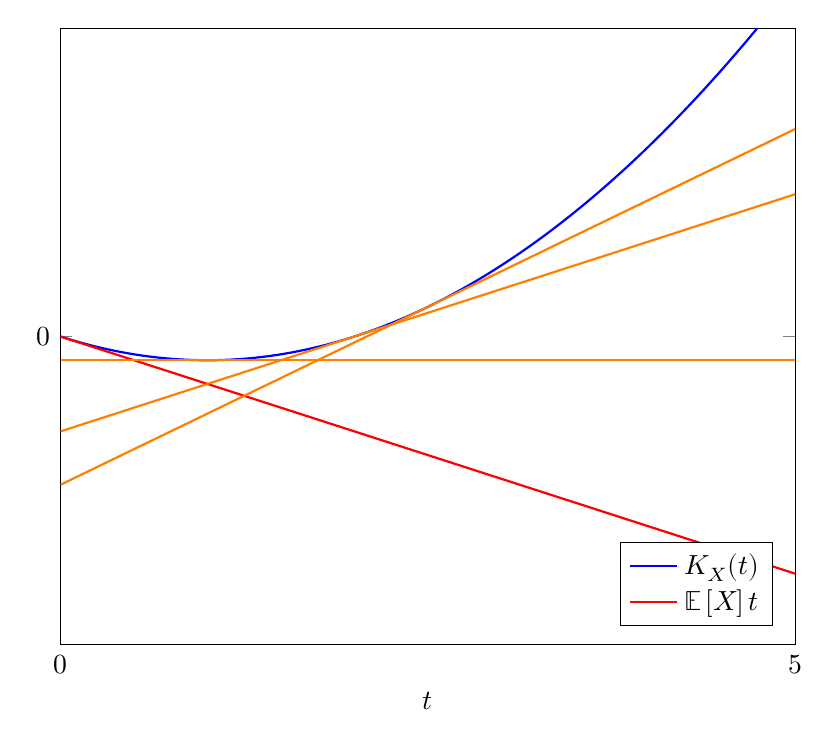
\begin{tikzpicture}
\begin{axis}[
    width=0.9\textwidth,
    xlabel=$t$,
    %ylabel=$K_X(x)$,
    xmin=0, xmax=5,
    ymin=-13, ymax=13,
    xtick={0,5},
    ytick={0},
    legend pos = south east
]
    \addplot[domain=0:5, samples=100, color=blue, thick] {-2*x+x^2};
    \addplot[domain=0:5, samples=100, color=red, thick] {-2*x};
    \addplot[domain=0:5, samples=100, color=orange, thick] {-1};
    \addplot[domain=0:5, samples=100, color=orange, thick] {2*(x-2) + 0};
    \addplot[domain=0:5, samples=100, color=orange, thick] {3*(x-5/2) - 5 + 25/4};
    \legend{$K_X(t)$, $\expt{X}t$}
\end{axis}
\end{tikzpicture}
\end{frame}

\begin{frame}{例(ベルヌーイ分布)}
\end{frame}

\begin{frame}{例(正規分布)}
%\small
\begin{align*}
p(x) &= \frac1{\sqrt{2\pi}} \mathrm{e}^{-\frac{(x-\mu)^2}{2\sigma^2}}
\end{align*}
\begin{align*}
M_X(t) &= \int_{-\infty}^\infty\frac1{\sqrt{2\pi}} \mathrm{e}^{-\frac{(x-\mu)^2}{2\sigma^2}} \mathrm{e}^{tx}\dx\\
 &= \int_{-\infty}^\infty\frac1{\sqrt{2\pi}} \mathrm{e}^{-\frac{(x-\mu -\sigma^2t)^2}{2\sigma^2}} \mathrm{e}^{\frac{(\mu+\sigma^2t)^2-\mu^2}{2\sigma^2}}\dx\\
&=\mathrm{e}^{\frac{(\mu+\sigma^2t)^2-\mu^2}{2\sigma^2}}
=\mathrm{e}^{\mu t + \frac{\sigma^2t^2}2}.
\end{align*}
\begin{align*}
K_X(t) &= \emm{\mu t + \frac{\sigma^2t^2}2}.\\
\end{align*}
\end{frame}

\begin{frame}{例(正規分布)}
\begin{align*}
K_X(t) &= \emm{\mu t + \frac{\sigma^2t^2}2}.\\
%\sup_{t>0} \left\{at - \left(\mu t + \frac{\sigma^2t^2}2\right)\right\} &= 
%\sup_{t>0} \left\{-\frac{\sigma^2}2 t\left(t-\frac{2(a-\mu)}{\sigma^2}\right) \right\}\\
% &= 
%\begin{cases}
%\emm{\frac{(a-\mu)^2}{2\sigma^2}}& a \ge \mu\\
%0&\text{otherwise.}
%\end{cases}
I(a)&=\sup_{t\in\mathbb{R}} \left\{at - \left(\mu t + \frac{\sigma^2t^2}2\right)\right\}\\
&= \sup_{t\in\mathbb{R}} \left\{-\frac{\sigma^2}2 t\left(t-\frac{2(a-\mu)}{\sigma^2}\right) \right\}\\
&=\emm{\frac{(a-\mu)^2}{2\sigma^2}}.
\end{align*}

\vspace{1em}
任意の$\epsilon>0$について
\begin{align*}
\Pr\left(\frac1N\sum_{k=1}^N X_k \ge \mu + \epsilon\right) &\le \mathrm{e}^{-\emm{\frac{\epsilon^2}{2\sigma^2}}N}\\
\Pr\left(\frac1N\sum_{k=1}^N X_k \le \mu - \epsilon\right) &\le \mathrm{e}^{-\emm{\frac{\epsilon^2}{2\sigma^2}}N}.
\end{align*}
\end{frame}

\begin{frame}{例(ポアソン分布)}
\begin{align*}
\Pr(X=k) &= \frac{\lambda^k\mathrm{e}^{-\lambda}}{k!}.
\end{align*}
\begin{align*}
M_X(t) &= \sum_{k\ge 0}\frac{\lambda^k\mathrm{e}^{-\lambda}}{k!} \mathrm{e}^{tk}\\
&= \mathrm{e}^{\lambda\mathrm{e}^t - \lambda}\\
K_X(t) &= \lambda(\mathrm{e}^t-1)
\end{align*}
\end{frame}

\begin{frame}{例(ポアソン分布)}
\begin{align*}
K_X(t) &= \lambda(\mathrm{e}^t-1)
\end{align*}
\begin{align*}
%\sup_{t>0}\left\{at - \lambda(\mathrm{e}^t-1)\right\}
I(a)&=\sup_{t\in\mathbb{R}}\left\{at - \lambda(\mathrm{e}^t-1)\right\}
\end{align*}
\begin{align*}
a-\lambda\mathrm{e}^{t^*} &= 0\iff t^* = \log \frac{a}{\lambda}
\end{align*}
\begin{align*}
%\sup_{t>0}\left\{at - \lambda(\mathrm{e}^t-1)\right\} &=
%\begin{cases}
%a\log\frac{a}{\lambda} -a + \lambda& a \ge \lambda\\
%0&\text{otherwise.}
%\end{cases}
I(a)&=\sup_{t\in\mathbb{R}}\left\{at - \lambda(\mathrm{e}^t-1)\right\}\\
 &= a\log\frac{a}{\lambda} -a + \lambda.
\end{align*}

\vspace{.5em}
%任意の$\epsilon>0$について
%任意の$c > 1$について
\begin{align*}
%\Pr\left(\frac1N\sum_{k=1}^N X_k \ge \lambda+\epsilon\right) &\le \mathrm{e}^{-\emm{((\lambda+\epsilon) \log\frac{\lambda+\epsilon}{\lambda} - \epsilon)}N}.
\Pr\left(\frac1N\sum_{k=1}^N X_k \ge c\lambda\right) &\le \mathrm{e}^{-\emm{\lambda\left(c\log c -c + 1 \right)}N}\qquad\forall c > 1\\
\Pr\left(\frac1N\sum_{k=1}^N X_k \le c\lambda\right) &\le \mathrm{e}^{-\emm{\lambda\left(c\log c -c + 1 \right)}N}\qquad\forall c < 1\\
\end{align*}
\end{frame}

\begin{frame}{例(指数分布)}
%\small
\begin{align*}
p(x) &= \lambda\mathrm{e}^{-\lambda x}\qquad\text{for}\quad x\ge 0
\end{align*}
\begin{align*}
M_X(t) &= \int_{0}^\infty \lambda\mathrm{e}^{-\lambda x} \mathrm{e}^{tx}\dx\\
&=\left[\frac{\lambda}{t-\lambda}\mathrm{e}^{(t-\lambda)x}\right]_0^{\infty}\\
&=\begin{cases}
\frac{\lambda}{\lambda-t}& t < \lambda\\
+\infty&\text{otherwise.}
\end{cases}
\end{align*}
\begin{align*}
K_X(t) &=
\begin{cases}
\log\frac{\lambda}{\lambda-t}& t < \lambda\\
+\infty&\text{otherwise.}
\end{cases}
\end{align*}
\end{frame}

\begin{frame}{例(指数分布)}
\small
\begin{align*}
K_X(t) &=
\begin{cases}
\log\frac{\lambda}{\lambda-t}& t < \lambda\\
+\infty&\text{otherwise.}
\end{cases}
\end{align*}
\begin{align*}
I(a) &= \sup_{t<\lambda} \left\{at - \log\frac{\lambda}{\lambda-t}\right\}
\end{align*}
\begin{align*}
a - \frac1{\lambda-t^*} &=0 \iff  t^* = \lambda-\frac1a
\end{align*}
\begin{align*}
I(a) &= \sup_{t<\lambda} \left\{at - \log\frac{\lambda}{\lambda-t}\right\}\\
&=
%\begin{cases}
a\lambda - 1 - \log(a\lambda)
%& a > \frac1\lambda\\
%0 & \text{otherwise.}
%\end{cases}
\end{align*}

%\vspace{.5em}
%任意の$\epsilon>0$について
%任意の$c > 1$について
\begin{align*}
%\Pr\left(\frac1N\sum_{k=1}^N X_k \ge \lambda+\epsilon\right) &\le \mathrm{e}^{-\emm{((\lambda+\epsilon) \log\frac{\lambda+\epsilon}{\lambda} - \epsilon)}N}.
\Pr\left(\frac1N\sum_{k=1}^N X_k \ge \frac{c}{\lambda}\right) &\le \mathrm{e}^{-\emm{(c-1-\log c)}N} \qquad\forall c>1\\
\Pr\left(\frac1N\sum_{k=1}^N X_k \ge \frac{c}{\lambda}\right) &\ge \mathrm{e}^{-\emm{(c-1-\log c)}N} \qquad\forall c<1.
\end{align*}
\end{frame}


\begin{frame}{大偏差原理 Lv1}
レート関数$I(a)$は\emm{最適な指数}であり、これ以上改善することはできない。証明は難しいので紹介しない。
\begin{theorem}[クラメールの定理]
\begin{align*}
\lim_{N\to\infty}\frac1N \log \Pr\left(\frac1N\sum_{k=1}^N X_k \ge a\right) &= -I(a) \qquad\forall a>\expt{X}\\
\lim_{N\to\infty}\frac1N \log \Pr\left(\frac1N\sum_{k=1}^N X_k \le a\right) &= -I(a) \qquad\forall a<\expt{X}
\end{align*}
\end{theorem}
\end{frame}

\begin{frame}{サブガウシアン}
キュムラントやレート関数が計算できればよいのだが、必ずしもそうとは限らない。

\vspace{1em}
$X$が\emm{サブガウシアン} $\stackrel{\mathrm{def}}{\iff}$ ある $s\ge0$が存在して
\begin{align*}
\expt{\mathrm{e}^{t(X-\expt{X})}} &\le \mathrm{e}^{\frac{s^2t^2}2}\qquad\forall t\in\mathbb{R}\\
\iff\expt{\mathrm{e}^{tX}} &\le \mathrm{e}^{\expt{E}t+\frac{s^2t^2}2\qquad\forall t\in\mathbb{R}}\\
\iff K_X(t) &\le {\expt{E}t+\frac{s^2t^2}2\qquad\forall t\in\mathbb{R}}\\
\end{align*}
\end{frame}

%\begin{frame}{大偏差原理 Lv2}
%\begin{theorem}[サノフの定理]
%\end{theorem}
%\end{frame}
\end{document}
